\begin{filecontents*}{figures/prodfunY.tikz}
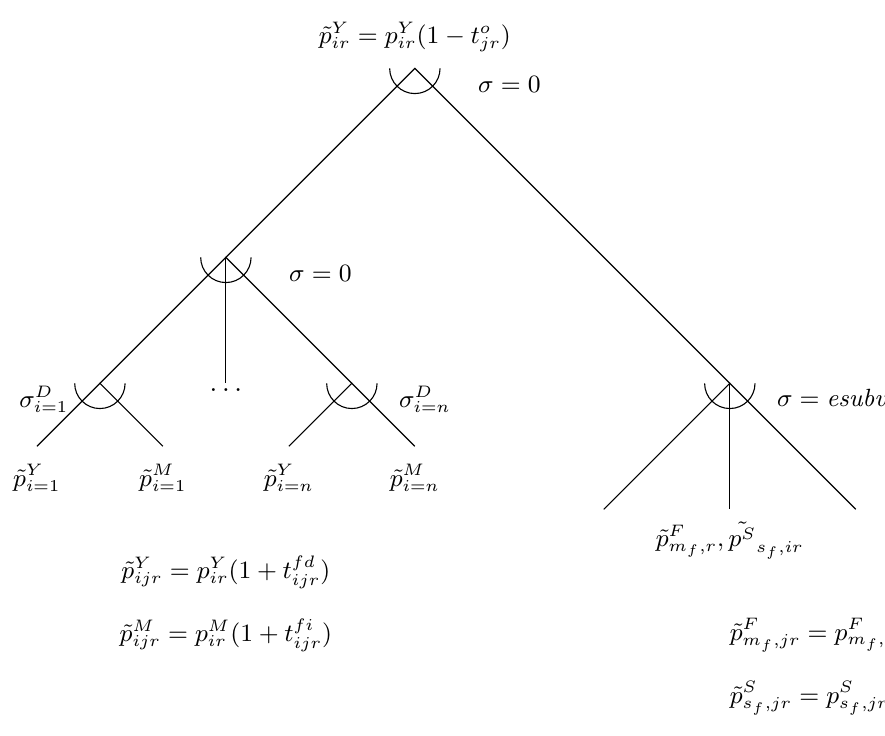
\begin{tikzpicture}[scale=0.8]
\node at (4,-1){\makebox(0,0)[c] {\small{$\tilde p^Y_{ijr} = p^Y_{ir} (1 + t^{fd}_{ijr})$}}};
\node at (4,-2){\makebox(0,0)[c]{\small{$\tilde p^M_{ijr} = p^M_{ir} (1 + t^{fi}_{ijr})$}}};
\node at (12,-2){\makebox(0,0)[l]{\small{$\tilde p^F_{m_f,jr} = p^F_{m_f,r} (1 + t^f_{m_f,jr})$}}};
\node at (12,-3){\makebox(0,0)[l]{\small{$\tilde p^S_{s_f,jr} = p^S_{s_f,jr} (1 + t^f_{s_f,jr})$}}};
%\node at (12,-4){\makebox(0,0)[l]{\small{$\sigma^D_i = \textit{esubd}_i$}}};
\node at (4,1.9){\makebox(0,0)[c]{$\ldots$}};
\node at (7,7.5){\makebox(0,0)[c]{\small{$\tilde p^Y_{ir} = p^Y_{ir} (1-t^o_{jr})$}}};
\node at (1,0.5){\makebox(0,0)[c]{\small{$\tilde p^Y_{i=1}$}}};
\node at (3,0.5){\makebox(0,0)[c]{\small{$\tilde p^M_{i=1}$}}};
\node at (5,0.5){\makebox(0,0)[c]{\small{$\tilde p^Y_{i=n}$}}};
\node at (7,0.5){\makebox(0,0)[c]{\small{$\tilde p^M_{i=n}$}}};
\node at (12,-0.5){\makebox(0,0)[c]{\small{$\tilde p^F_{m_f,r},\tilde{p^S}_{s_f,ir}$}}};
\node at (8.5,6.75){\makebox(0,0)[c]{\small{$\sigma=0$}}};
\node at (5.5,3.75){\makebox(0,0)[c]{\small{$\sigma=0$}}};
\node at (1.5,1.75){\makebox(0,0)[r]{\small{$\sigma^D_{i=1}$}}};
\node at (6.75,1.75){\makebox(0,0)[l]{\small{$\sigma^D_{i=n}$}}};
\node at (12.75,1.75){\makebox(0,0)[l]{\small{$\sigma=\textit{esubva}_i$}}};
\draw (2.4,2) arc (0:-180:0.4cm);
\draw (4.4,4) arc (0:-180:0.4cm);
\draw (6.4,2) arc (0:-180:0.4cm);
\draw (7.4,7) arc (0:-180:0.4cm);
\draw (12.4,2) arc (0:-180:0.4cm);
\draw (1,1)--(2,2)--(3,1);
\draw (5,1)--(6,2)--(7,1);
\draw (2,2)--(4,4)--(6,2);
\draw (4,4)--(4,2);
\draw (4,4)--(7,7)--(12,2);
\draw (10,0)--(12,2)--(14,0);
\draw (12,2)--(12,0);
\end{tikzpicture}
\end{filecontents*}

\begin{filecontents*}{figures/prodfunDX.tikz}
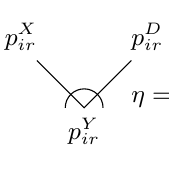
\begin{tikzpicture}[scale=0.6]
\draw (1,2)--(2,1)--(3,2);
\draw (2.4,1) arc (0:180:0.4cm);
\node at (3,1.25){\makebox(0,0)[l]{\small{$\eta=\textit{etrndx}_{i}$}}};
\node at (1,2.5){\makebox(0,0)[r]{\small{$p^X_{ir}$}}};
\node at (3,2.5){\makebox(0,0)[l]{\small{$p^D_{ir}$}}};
\node at (2,0.5){\makebox(0,0)[c]{\small{$p^Y_{ir}$}}};
\end{tikzpicture}
\end{filecontents*}

\begin{filecontents*}{figures/prodfunA.tikz}
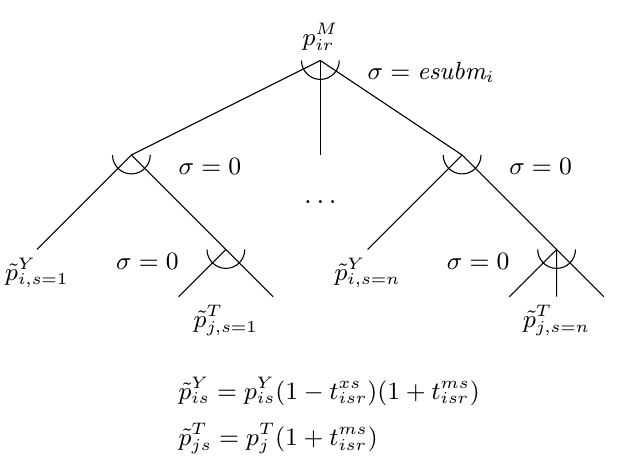
\begin{tikzpicture}[scale=0.6]
\node at (8,5.75){\makebox(0,0)[l]{\small{$\sigma=\textit{esubm}_i$}}};
\node at (4,3.75){\makebox(0,0)[l]{\small{$\sigma=0$}}};
\node at (11,3.75){\makebox(0,0)[l]{\small{$\sigma=0$}}};
\node at (4,1.75){\makebox(0,0)[r]{\small{$\sigma=0$}}};
\node at (11,1.75){\makebox(0,0)[r]{\small{$\sigma=0$}}};
\draw (1,2)--(3,4)--(7,6)--(10,4)--(12,2)--(13,1);
\draw (3,4)--(5,2);
\draw (4,1)--(5,2)--(6,1);
\draw (7,6)--(7,4);
\draw (8,2)--(10,4);
\draw (11,1)--(12,2)--(12,1);
\draw (3.4,4) arc (0:-180:0.4cm);
\draw (7.4,6) arc (0:-180:0.4cm);
\draw (5.4,2) arc (0:-180:0.4cm);
\draw (10.4,4) arc (0:-180:0.4cm);
\draw (12.4,2) arc (0:-180:0.4cm);
\node at (7,6.5){\makebox(0,0)[c]{\small{$p^M_{ir}$}}};
\node at (1,1.5){\makebox(0,0)[c]{\small{$\tilde{p}^Y_{i,s=1}$}}};
\node at (5,0.5){\makebox(0,0)[c]{\small{$\tilde{p}^T_{j,s=1}$}}};
\node at (8,1.5){\makebox(0,0)[c]{\small{$\tilde{p}^Y_{i,s=n}$}}};
\node at (12,0.5){\makebox(0,0)[c]{\small{$\tilde{p}^T_{j,s=n}$}}};
\node at (7,3){\makebox(0,0)[c]{$\ldots$}};
\node at (4,-1){\makebox(0,0)[l]{\small{$\tilde{p}^Y_{is} = p^Y_{is} (1 - t^{xs}_{isr})(1 + t^{ms}_{isr})$}}};
\node at (4,-2){\makebox(0,0)[l]{\small{$\tilde{p}^T_{js} = p^T_j (1 + t^{ms}_{isr})$}}};
\end{tikzpicture}
\end{filecontents*}


\begin{filecontents*}{figures/gtapflowchart.tikz}
\tikzset{%
  block/.style    = {draw, thick, rectangle, minimum height = 3em,
    minimum width = 3em},
  sum/.style      = {draw, circle, node distance = 2cm}, % Adder
  input/.style    = {coordinate}, % Input
  output/.style   = {coordinate} % Output
}
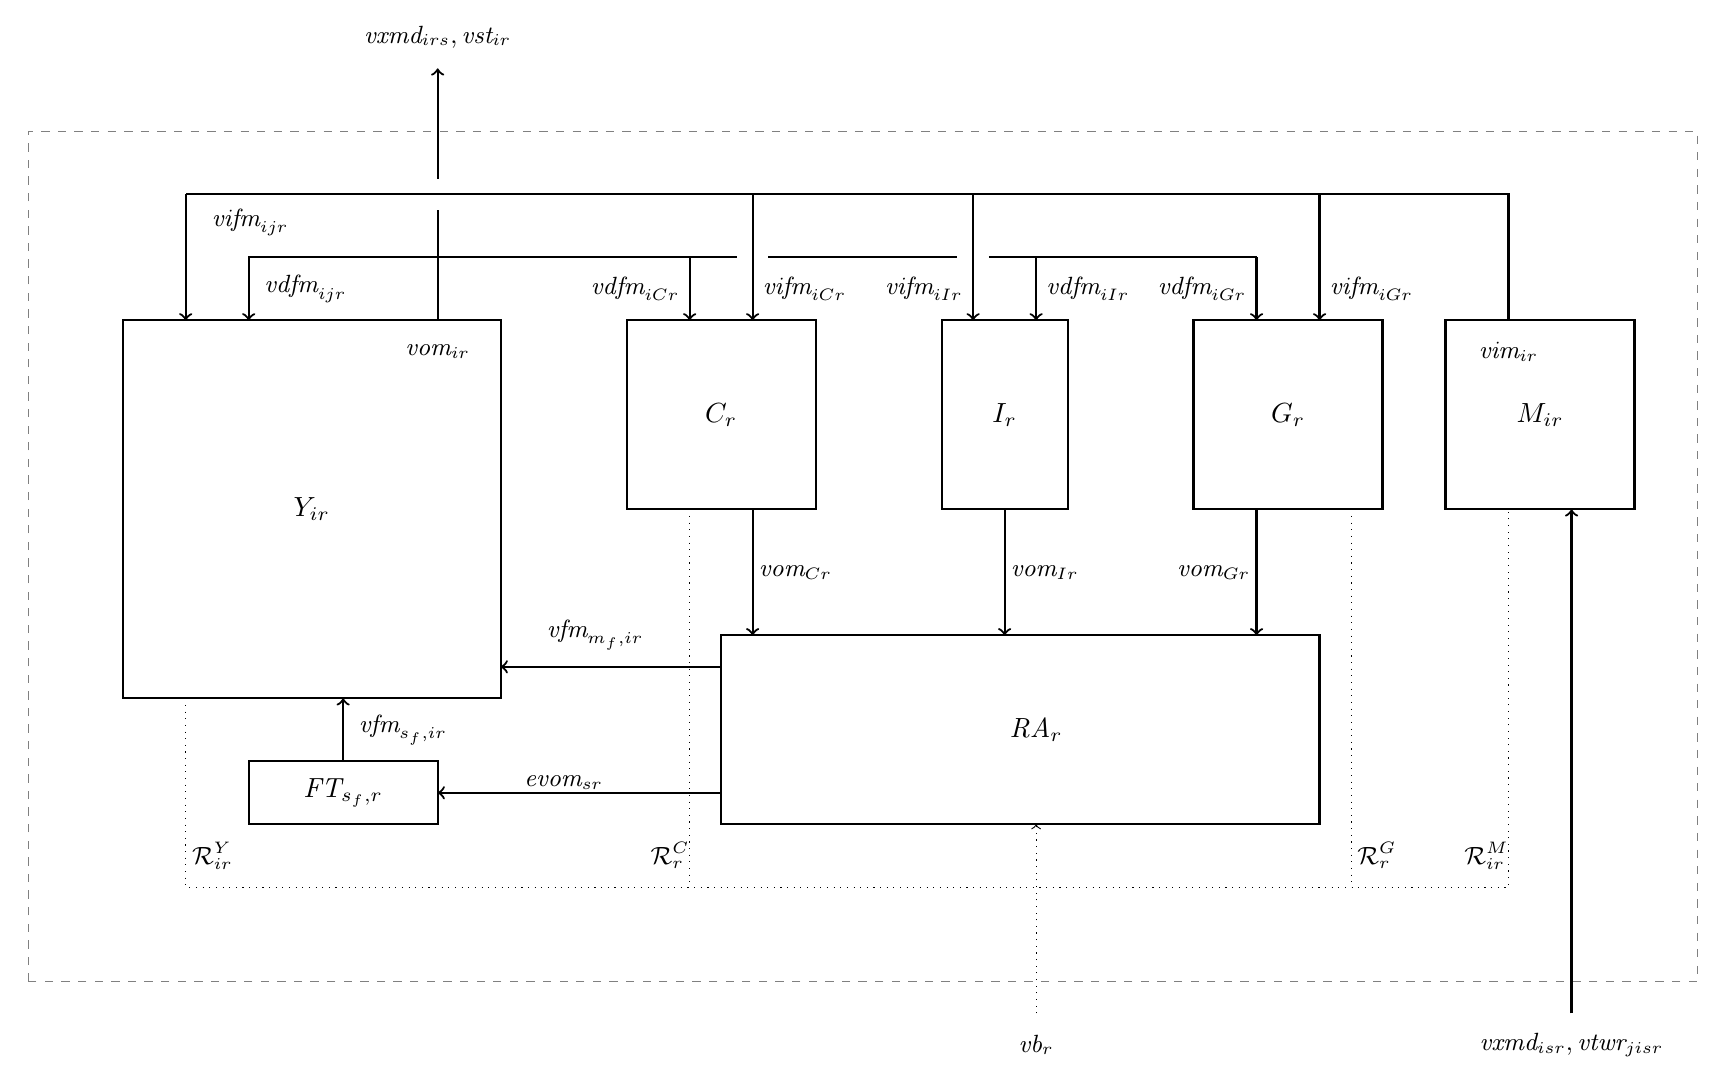
\begin{tikzpicture}[auto, thick, scale=0.8]
\draw[gray,thin,dashed] (-2.5,-0.5) rectangle (24,13);

\draw (-1,4)  rectangle (5,10);
\node at (2,7) {$Y_{ir}$};

\draw (1,2)   rectangle (4,3);
\node at (2.5,2.5) {$\textit{FT}_{s_{f},r}$};

\draw (8.5,2) rectangle (18,5);
\node at (13.5,3.5)  {$\textit{RA}_r$};

\draw (7,7) rectangle (10,10);
\node at (8.5,8.5) {$C_r$};

\draw (12,7) rectangle (14,10);
\node at (13,8.5) {$I_r$};

\draw (16,7) rectangle (19,10);
\node at (17.5,8.5) {$G_r$};

\draw (20,7) rectangle (23,10);
\node at (21.5,8.5) {$M_{ir}$};


\node [right] at (0.25,11.55) {\small{$\textit{vifm}_{ijr}$}};


\draw[thin,dotted] (0,4)--(0,1)--(21,1)--(21,7);  % Y to M (GOVT)
\node at (0.1,1.5) {\makebox(0,0)[l]{\small{$\mathcal{R}^Y_{ir}$}}};

\draw[thin,dotted] (8,7)--(8,1);              % C to GOVT
\node at (8,1.5) {\makebox(0,0)[r]{\small{$\mathcal{R}^C_r$}}};

%\dottedline{0.1}(13,7)(13,1)           % I to GOVT

\draw[->,thin,dotted] (13.5,-1)--(13.5,2);       % G to GOVT
\node at (13.5,-1.5){\makebox(0,0)[c]{\small{$\textit{vb}_r$}}};

\node at (18.6,1.5) {\makebox(0,0)[l]{\small{$\mathcal{R}^G_r$}}};
\node at (21,1.5) {\makebox(0,0)[r]{\small{$\mathcal{R}^M_{ir}$}}};

\draw[thin,dotted] (18.5,7)--(18.5,1);        % M to GOVT
%\draw[thin,dotted] (10.5,2)--(10.5,1);        % HH to GOVT

\draw (21,10)--(21,12)--(0,12);               % M to market
\node at (21,9.5){\makebox(0,0)[c]{\small{$\textit{vim}_{ir}$}}};
\draw (4,10)--(4,11)--(8.75,11);              % Y to market
\node at (4,9.5){\makebox(0,0)[c]{\small{$\textit{vom}_{ir}$}}};

\draw (4,11)--(4,11.75);             % Y to ROW
\draw (4,12.25)--(4,13.75);
\draw [->] (4,13.75)--(4,14);
\node at (4,14.5){\makebox(0,0)[c]{\small{$\textit{vxmd}_{irs},\textit{vst}_{ir}$}}};
\draw (4,11)--(1,11)--(1,10.25);              % Y to Y
\draw [->] (1,10.25)--(1,10);      % Y to Y
\node at (1.25,10.5) {\makebox(0,0)[l]{\small{$\textit{vdfm}_{ijr}$}}};

\draw  (9.25,11)--(12.25,11);            % Y to market
\draw  (12.75,11)--(17,11);            % Y to market

\draw  (22,-1)--(22,6.75);            % ROW to M
\draw [->] (22,6.75)--(22,7);
%\put(22,7.5){\makebox(0,0)[c]{\small{$p^Y_{is}, p^T_j$}}}

\node at (22,-1.5) {\makebox(0,0)[c]{\small{$\textit{vxmd}_{isr},\textit{vtwr}_{jisr}$}}};
\draw[->] (0,12)--(0,10);     % M to Y

\draw[->] (8,11)--(8,10);     % Y to C
\node [left]  at (8,10.5) {\small{$\textit{vdfm}_{iCr}$}};

\draw[->] (9,12)--(9,10);     % M to C
\node [right] at (9,10.5) {\small{$\textit{vifm}_{iCr}$}};

\draw[->] (12.5,12)--(12.5,10);   % M to I
\node [left] at (12.5,10.5) {\small{$\textit{vifm}_{iIr}$}};

\draw[->] (13.5,11)--(13.5,10);   % Y to I
\node [right] at (13.5,10.5) {\small{$\textit{vdfm}_{iIr}$}};

\node [left]  at (17,10.5) {\small{$\textit{vdfm}_{iGr}$}};
\node [right] at (18,10.5) {\small{$\textit{vifm}_{iGr}$}};
\draw[->] (17,11)--(17,10);   % Y to G
\draw[->] (18,12)--(18,10);   % M to G

\draw (9,7)--(9,5.25);          % C to HH
%\put(9,7.5){\makebox(0,0)[c]{\small{$p^C_{r}$}}}
\node  at (9.1,6){\makebox(0,0)[l]{\small{$\textit{vom}_{Cr}$}}};

\draw (13,7)--(13,5.25);        % I to HH
%\put(12,7.5){\makebox(0,0)[c]{\small{$p^Y_{\mbox{\textsc{cgd}},r}$}}}
\node at (13.1,6){\makebox(0,0)[l]{\small{$\textit{vom}_{Ir}$}}};
\draw (17,7)--(17,5.25);        % G to GOVT
%\put(17,7.5){\makebox(0,0)[c]{\small{$p^G_{r}$}}}

\draw (5.25,4.5)--(8.5,4.5);            % HH to Y
\draw[->] (5.25,4.5)--(5,4.5);     % HH to Y
\node at (6.5,5.0){\makebox(0,0)[c]{\small{$\textit{vfm}_{m_{f},ir}$}}};
%\put(4.75,3.5){\makebox(0,0)[r]{\small{$p^F_{fr},p^S_{fir}$}}}

\draw[<-] (4,2.5)--(8.5,2.5);     % HH to FT
\node[above] at (6,2.5) {\makebox(0,0)[c]{\small{$\textit{evom}_{sr}$}}};

\draw (2.5,3)--(2.5,3.75);              % FT to Y
\draw[->] (2.5,3.75)--(2.5,4);      % HH to FT
\node at (2.75,3.5){\makebox(0,0)[l]{\small{$\textit{vfm}_{s_{f},ir}$}}};

\draw[->] (9,5.25)--(9,5);       % C to HH
\draw[->] (13,5.25)--(13,5);      % I to HH

\draw[->] (17,5.25)--(17,5);      % G to GOVT
\node at (16.9,6){\makebox(0,0)[r]{\small{$\textit{vom}_{Gr}$}}};
\end{tikzpicture}
\end{filecontents*}

\begin{filecontents*}{figures/prodfunC.tikz}
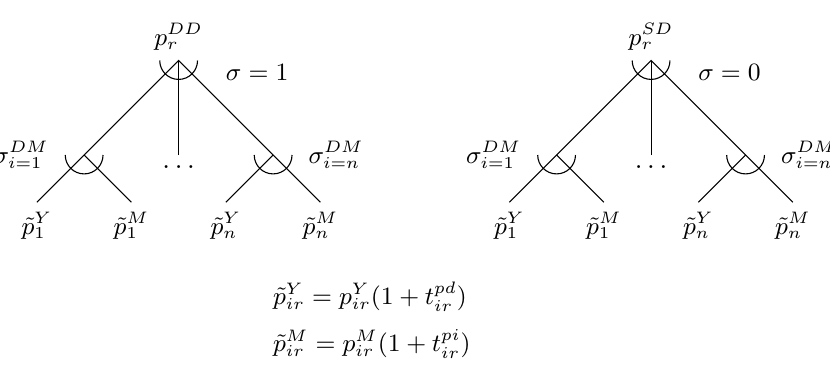
\begin{tikzpicture}[scale=0.6]
\draw(1,1)--(2,2)--(4,4)--(6,2)--(7,1);
\draw(2,2)--(3,1);
\draw(5,1)--(6,2);
\draw (4,2)--(4,4);
\node at (4,1.75){\makebox(0,0)[c]{$\ldots$}};
\draw (4.4,4) arc (0:-180:0.4cm);
\draw (2.4,2) arc (0:-180:0.4cm);
\draw (6.4,2) arc (0:-180:0.4cm);
\node at (5,3.75){\makebox(0,0)[l]{\small{$\sigma=1$}}};
\node at (1.25,2){\makebox(0,0)[r]{\small{$\sigma^{DM}_{i=1}$}}};
\node at (6.75,2){\makebox(0,0)[l]{\small{$\sigma^{DM}_{i=n}$}}};
\node at (1,0.5){\makebox(0,0)[c]{\small{$\tilde{p}^Y_{1}$}}};
\node at (3,0.5){\makebox(0,0)[c]{\small{$\tilde{p}^M_{1}$}}};
\node at (5,0.5){\makebox(0,0)[c]{\small{$\tilde{p}^Y_{n}$}}};
\node at (7,0.5){\makebox(0,0)[c]{\small{$\tilde{p}^M_{n}$}}};
\node at (4,4.5){\makebox(0,0)[c]{\small{$p^{DD}_r$}}};
\node at (6,-1){\makebox(0,0)[l]{\small{$\tilde{p}^Y_{ir} = p^Y_{ir} (1 + t^{pd}_{ir})$}}};
\node at (6,-2){\makebox(0,0)[l]{\small{$\tilde{p}^M_{ir} = p^M_{ir} (1 + t^{pi}_{ir})$}}};
\draw(11,1)--(12,2)--(14,4)--(16,2)--(17,1);
\draw(12,2)--(13,1);
\draw(15,1)--(16,2);
\draw (14,2)--(14,4);
\node at (14,1.75){\makebox(0,0)[c]{$\ldots$}};
\draw (14.4,4) arc (0:-180:0.4cm);
\draw (12.4,2) arc (0:-180:0.4cm);
\draw (16.4,2) arc (0:-180:0.4cm);
\node at (15,3.75){\makebox(0,0)[l]{\small{$\sigma=0$}}};
\node at (11.25,2){\makebox(0,0)[r]{\small{$\sigma^{DM}_{i=1}$}}};
\node at (16.75,2){\makebox(0,0)[l]{\small{$\sigma^{DM}_{i=n}$}}};
\node at (11,0.5){\makebox(0,0)[c]{\small{$\tilde{p}^Y_{1}$}}};
\node at (13,0.5){\makebox(0,0)[c]{\small{$\tilde{p}^M_{1}$}}};
\node at (15,0.5){\makebox(0,0)[c]{\small{$\tilde{p}^Y_{n}$}}};
\node at (17,0.5){\makebox(0,0)[c]{\small{$\tilde{p}^M_{n}$}}};
\node at (14,4.5){\makebox(0,0)[c]{\small{$p^{SD}_r$}}};
\end{tikzpicture}
\end{filecontents*}

\begin{filecontents*}{figures/prodfunFT.tikz}
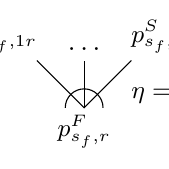
\begin{tikzpicture}[scale=0.6]
\draw (1,2)--(2,1)--(3,2);
\draw (2,1)--(2,2);
\draw (2.4,1) arc (0:180:0.4cm);
\node at (2,2.25){\makebox(0,0)[c]{$\ldots$}};
\node at (3,1.25){\makebox(0,0)[l]{\small{$\eta=\textit{etrae}_{s_{f}}$}}};
\node at (1,2.5){\makebox(0,0)[r]{\small{$p^S_{s_{f},1r}$}}};
\node at (3,2.5){\makebox(0,0)[l]{\small{$p^S_{s_{f},nr}$}}};
\node at (2,0.5){\makebox(0,0)[c]{\small{$p^F_{s_{f},r}$}}};
\end{tikzpicture}
\end{filecontents*}

\begin{filecontents*}{figures/prodfunYT.tikz}
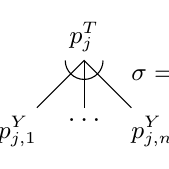
\begin{tikzpicture}[scale=0.6]
\draw(1,1)--(2,2)--(3,1);
\draw(2,1)--(2,2);
\draw (2.4,2) arc (0:-180:0.4cm);
\node at (2,0.75){\makebox(0,0)[c]{$\ldots$}};
\node at (3,1.75){\makebox(0,0)[l]{\small{$\sigma=1$}}};
\node at (1,0.5){\makebox(0,0)[r]{\small{$p^Y_{j,1}$}}};
\node at (3,0.5){\makebox(0,0)[l]{\small{$p^Y_{j,n}$}}};
\node at (2,2.5){\makebox(0,0)[c]{\small{$p^T_j$}}};
\end{tikzpicture}
\end{filecontents*}

\begin{filecontents*}{figures/prodfunG.tikz}
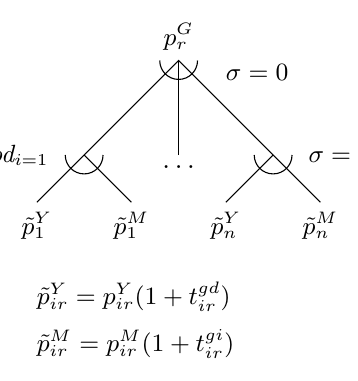
\begin{tikzpicture}[scale=0.6]
\draw(1,1)--(2,2)--(4,4)--(6,2)--(7,1);
\draw(2,2)--(3,1);
\draw(5,1)--(6,2);
\draw (4,2)--(4,4);
\node at (4,1.75){\makebox(0,0)[c]{$\ldots$}};
\draw (4.4,4) arc (0:-180:0.4cm);
\draw (2.4,2) arc (0:-180:0.4cm);
\draw (6.4,2) arc (0:-180:0.4cm);
\node at (5,3.75){\makebox(0,0)[l]{\small{$\sigma=0$}}};
\node at (1.25,2){\makebox(0,0)[r]{\small{$\sigma=\textit{esubd}_{i=1}$}}};
\node at (6.75,2){\makebox(0,0)[l]{\small{$\sigma=\textit{esubd}_{i=n}$}}};
\node at (1,0.5){\makebox(0,0)[c]{\small{$\tilde{p}^Y_{1}$}}};
\node at (3,0.5){\makebox(0,0)[c]{\small{$\tilde{p}^M_{1}$}}};
\node at (5,0.5){\makebox(0,0)[c]{\small{$\tilde{p}^Y_{n}$}}};
\node at (7,0.5){\makebox(0,0)[c]{\small{$\tilde{p}^M_{n}$}}};
\node at (4,4.5){\makebox(0,0)[c]{\small{$p^G_r$}}};
\node at (1,-1){\makebox(0,0)[l]{\small{$\tilde{p}^Y_{ir} = p^Y_{ir}
(1 + t^{gd}_{ir})$}}};
\node at (1,-2){\makebox(0,0)[l]{\small{$\tilde{p}^M_{ir} = p^M_{ir}
(1 + t^{gi}_{ir})$}}};
\end{tikzpicture}
\end{filecontents*}

\begin{filecontents*}{figures/figure9a.tikz}
\begin{tikzpicture}
 \pgfplotsset{filter discard warning=false}
\begin{axis}[
%  legend cell align=left,
%  height=0.4\textheight,
  xlabel shift = 0.05in,
  ylabel shift = -0.05in,
  xlabel={Quantity ($q$)},
  ylabel={Price ($p$)},
  axis line style={->},
  axis x line* = bottom,
  axis y line = left,
  grid = major,
  grid style={dashed, gray!30},
  xmin = 0,
  xmax = 3,
  ymin = 0.8,
  ymax = 1.4]
\addplot[color=red, thick, solid] table [y=p, x=q]{figures/figure9.data};
\addplot[color=blue, thick,  dashed] table [y=pref, x=q]{figures/figure9.data};
\node[circle,label={135:$b$},fill=black,scale=0.3] at (axis cs:1,1)     {};
\node[circle,label={ 45:$a$},fill=black,scale=0.3] at (axis cs:1,1.2)   {};
\node[circle,label={-135:$c$},fill=black,scale=0.3] at (axis cs:2.48832,1) {};
\end{axis}
\end{tikzpicture}
\end{filecontents*}{figures/figure9a.tikz}

\begin{filecontents*}{figures/figure9b.tikz}
\begin{tikzpicture}
\pgfplotsset{filter discard warning=false}
\begin{axis}[
%  legend cell align=left,
%  height=0.4\textheight,
  xlabel shift = 0.05in,
  ylabel shift = -0.05in,
  xlabel={Quantity ($q$)},
  ylabel={Price ($p$)},
  axis line style={->},
  axis x line* = bottom,
  axis y line = left,
  grid = major,
  grid style={dashed, gray!30},
  xmin = 0,
  xmax = 3,
  ymin = 0.8,
  ymax = 1.4]
\addplot[color=red,  thick, solid] table [y=p, x=d]{figures/figure9.data};
\addplot[color=blue, thick, dashed] table [y=p, x=s]{figures/figure9.data};
\addplot[color=red,  thin,  solid] table [y=p, x=q]{figures/figure9.data};
\addplot[color=blue, thin,  dashed] table [y=pref, x=q]{figures/figure9.data};
\draw [color=black, thin, dashed] (axis cs:2.48832,0.8) -- (axis cs:2.48832,1.18) -- (axis cs:0,1.18);
\node[circle,label={135:$b$},fill=black,scale=0.3] at (axis cs:1,1)     {};
\node[circle,label={ 45:$a$},fill=black,scale=0.3] at (axis cs:1,1.2)   {};
\node[circle,label={-135:$c$},fill=black,scale=0.3] at (axis cs:2.48832,1) {};
\node[circle,label={-45:$d$},fill=black,scale=0.3] at (axis cs:2.48832,1.18) {};
\end{axis}
\end{tikzpicture}
\end{filecontents*}{figures/figure9b.tikz}

%	The data presented here has been copied from ExportElasticity.xlsx
%	in the LaTeX/figures directory:

\begin{filecontents}{figures/figure9.data}
p	q		pref	d		s
nan	0		1.0	nan		nan
1.3	0.670176922	1.0	0.01827657	4.29554847
1.29	0.696558632	1.0	0.026889132	4.115165249
1.28	0.724196434	1.0	0.039679283	3.941040905
1.27	0.753160657	1.0	0.058732198	3.773004634
1.26	0.783526166	1.0	0.087203727	3.610889011
1.25	0.815372698	1.0	0.129885794	3.454529941
1.24	0.848785212	1.0	0.194078776	3.303766628
1.23	0.883854288	1.0	0.290942208	3.158441529
1.22	0.92067654	1.0	0.437593406	3.018400312
1.21	0.959355078	1.0	0.660379809	2.883491822
1.2	1		1.0	1		2.753568034
1.19	1.042728931	1.0	1.519547333	2.62848402
1.18	1.087667605	1.0	2.317191555	2.508097903
1.17	1.134950503	1.0	3.546248908	2.39227082
1.16	1.184721539	1.0	5.447068553	2.280866886
1.15	1.237134814	1.0	8.397891991	2.173753149
1.14	1.292355435	1.0	nan		2.070799555
1.13	1.350560404	1.0	nan		1.971878908
1.12	1.411939594	1.0	nan		1.876866831
1.11	1.476696809	1.0	nan		1.785641729
1.1	1.545050947	1.0	nan		1.698084751
1.09	1.617237267	1.0	nan		1.614079749
1.08	1.693508781	1.0	nan		1.533513242
1.07	1.77413777	1.0	nan		1.456274381
1.06	1.859417457	1.0	nan		1.382254907
1.05	1.949663831	1.0	nan		1.311349117
1.04	2.045217658	1.0	nan		1.243453825
1.03	2.14644669	1.0	nan		1.178468328
1.02	2.253748089	1.0	nan		1.116294364
1.01	2.3675511	1.0	nan		1.056836081
1	2.48832		1.0	nan		1
0.99	2.616557345	1.0	nan		0.945694974
0.98	2.752807557	1.0	nan		0.893832159
0.97	2.897660889	1.0	nan		0.844324973
0.96	3.051757813	1.0	nan		0.797089063
0.95	3.215793876	1.0	nan		0.75204227
0.94	3.390525088	1.0	nan		0.709104592
0.93	3.576773897	1.0	nan		0.668198151
0.92	3.775435834	1.0	nan		0.629247158
0.91	3.987486894	1.0	nan		0.592177878
0.9	4.21399177	1.0	nan		0.556918595
0.89	4.456113017	1.0	nan		0.523399581
0.88	4.715121297	1.0	nan		0.491553056
0.87	4.992406813	1.0	nan		0.461313164
0.86	5.289492114	1.0	nan		0.43261593
0.85	5.608046444	1.0	nan		0.405399231
0.84	5.949901827	1.0	nan		0.379602765
\end{filecontents}
